\documentclass[tikz, border=1cm]{standalone}
\usetikzlibrary{fit}

% color shades in HEX
\definecolor{level-2}{HTML}{0082ce}
\definecolor{level-1}{HTML}{009bf5}
\definecolor{level0}{HTML}{31b3ff}
\definecolor{level+1}{HTML}{58c1ff}
\definecolor{level+2}{HTML}{7fd0ff}

\begin{document}

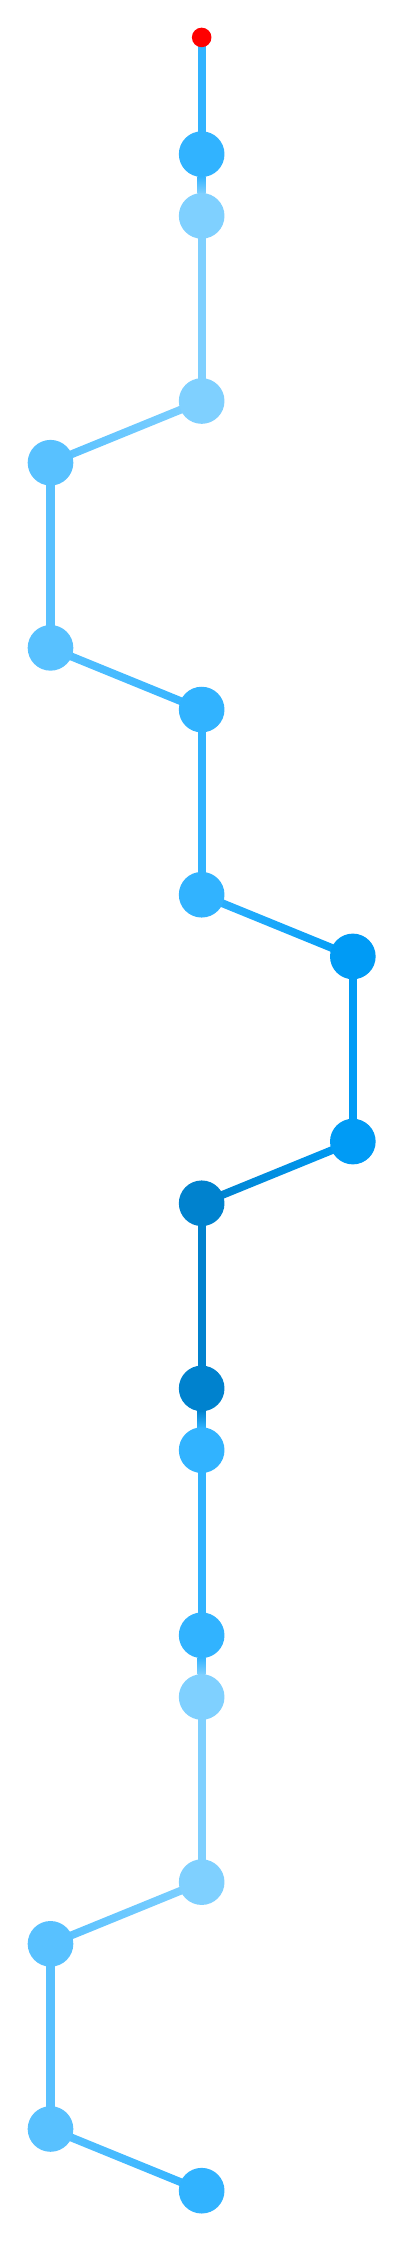
\begin{tikzpicture} % 'yz' side view, with +x coming out of the page

%% coordinates from file
\coordinate (h01)  at ( 0.00000000000000, 28.52186817612748);
\coordinate (si01) at ( 0.00000000000000, 27.03947817579129);
\coordinate (si02) at ( 0.00000000000000, 26.25572518518865);
\coordinate (si03) at ( 0.00000000000000, 23.90446621338074);
\coordinate (si04) at (-1.91979491135683, 23.12071322277810);
\coordinate (si05) at (-1.91979491135683, 20.76945425097014);
\coordinate (si06) at ( 0.00000000000000, 19.98570126036750);
\coordinate (si07) at ( 0.00000000000000, 17.63444228855953);
\coordinate (si08) at ( 1.91979491135683, 16.85068929795689);
\coordinate (si09) at ( 1.91979491135683, 14.49943032614898);
\coordinate (si10) at ( 0.00000000000000, 13.71567733554634);
\coordinate (si11) at ( 0.00000000000000, 11.36441836373838);
\coordinate (si12) at ( 0.00000000000000, 10.58066537313574);
\coordinate (si13) at ( 0.00000000000000,  8.22940640132778);
\coordinate (si14) at ( 0.00000000000000,  7.44565341072513);
\coordinate (si15) at ( 0.00000000000000,  5.09439443891722);
\coordinate (si16) at (-1.91979491135683,  4.31064144831458);
\coordinate (si17) at (-1.91979491135683,  1.95938247650662);
\coordinate (si18) at ( 0.00000000000000,  1.17562948590398);

%% bonds
\draw [line width=3pt, level0] (h01.center) -- (si01.center);
\path [rotate=0, top color=level0, bottom color=level+2]
        ([shift={(-0.05, -0.28)}] si01) rectangle ([shift={(0.05, 0.28)}] si02); 
\draw [line width=3pt, level+2] (si02.center) -- (si03.center);
\path [rotate=22.2, left color=level+1, right color=level+2]
        ([shift={(-0.05, 0.05)}] si03) rectangle ([shift={(0.05, -0.05)}] si04); 
\draw [line width=3pt, level+1] (si04.center) -- (si05.center);
\path [rotate=-22.2, left color=level+1, right color=level0]
        ([shift={(-0.05, 0.05)}] si05) rectangle ([shift={(0.05, -0.05)}] si06); 
\draw [line width=3pt, level0] (si06.center) -- (si07.center);
\path [rotate=-22.2, left color=level0, right color=level-1]
        ([shift={(-0.05, 0.05)}] si07) rectangle ([shift={(0.05, -0.05)}] si08); 
\draw [line width=3pt, level-1] (si08.center) -- (si09.center);
\path [rotate=22.2, left color=level-2, right color=level-1]
        ([shift={(-0.05, 0.05)}] si09) rectangle ([shift={(0.05, -0.05)}] si10); 
\draw [line width=3pt, level-2] (si10.center) -- (si11.center);
\path [rotate=0, top color=level-2, bottom color=level0]
        ([shift={(-0.05, -0.28)}] si11) rectangle ([shift={(0.05, 0.28)}] si12);
\draw [line width=3pt, level0] (si12.center) -- (si13.center);
\path [rotate=0, top color=level0, bottom color=level+2]
        ([shift={(-0.05, -0.28)}] si13) rectangle ([shift={(0.05, 0.28)}] si14);
\draw [line width=3pt, level+2] (si14.center) -- (si15.center);
\path [rotate=22.2, left color=level+1, right color=level+2]
        ([shift={(-0.05, 0.05)}] si15) rectangle ([shift={(0.05, -0.05)}] si16); 
\draw [line width=3pt, level+1] (si16.center) -- (si17.center);
\path [rotate=-22.2, left color=level+1, right color=level0]
        ([shift={(-0.05, 0.05)}] si17) rectangle ([shift={(0.05, -0.05)}] si18); 

%% atoms
\node [scale=0.75, circle, fill=red] at (h01) {};
\node [scale=1.75, circle, fill=level0 ] at (si01) {};
\node [scale=1.75, circle, fill=level+2] at (si02) {};
\node [scale=1.75, circle, fill=level+2] at (si03) {};
\node [scale=1.75, circle, fill=level+1] at (si04) {};
\node [scale=1.75, circle, fill=level+1] at (si05) {};
\node [scale=1.75, circle, fill=level0 ] at (si06) {};
\node [scale=1.75, circle, fill=level0 ] at (si07) {};
\node [scale=1.75, circle, fill=level-1] at (si08) {};
\node [scale=1.75, circle, fill=level-1] at (si09) {};
\node [scale=1.75, circle, fill=level-2] at (si10) {};
\node [scale=1.75, circle, fill=level-2] at (si11) {};
\node [scale=1.75, circle, fill=level0 ] at (si12) {};
\node [scale=1.75, circle, fill=level0 ] at (si13) {};
\node [scale=1.75, circle, fill=level+2] at (si14) {};
\node [scale=1.75, circle, fill=level+2] at (si15) {};
\node [scale=1.75, circle, fill=level+1] at (si16) {};
\node [scale=1.75, circle, fill=level+1] at (si17) {};
\node [scale=1.75, circle, fill=level0 ] at (si18) {};
\end{tikzpicture}



\end{document}
